% =============================================================================
% Pillar 3 — Iter 99: per-step decomposition for G∈{2,4,8,16}
% Driver: scripts/group_size_iter99.py
% Inputs:  experiments/results/groupsize_zvf_sweep.json
% Outputs: experiments/results/group_size_iter99_signal_amplitude.tsv
%          experiments/results/group_size_iter99_snr_at_g.tsv
%          experiments/results/group_size_iter99_noise_floor.tsv
%          experiments/results/group_size_iter99_trajectory_equiv.tsv
%          figures/group_size_iter99.pdf
% =============================================================================
\section{Iter 99 -- Per-step decomposition of the G=4 vs G=32 question}
\label{sec:group-size-iter99}

\paragraph{Motivation.}
Wu et al.~\cite{wu2025grpo_dpo}'s algebraic reduction says GRPO is
implicitly DPO once Monte Carlo (MC) averaging is factored out: across
$G$ only the MC noise on the per-step group advantage changes, not the
underlying signal.  We sharpen the test on the existing
12-run sweep ($G{\in}\{2,4,8,16\}\times 3$ seeds, 40 steps,
Qwen2.5-0.5B / arithmetic) by decomposing the per-step reward trace
into the four components that algebraic equivalence is obliged to
either satisfy or break: (A) advantage-signal amplitude via
$1-\mathrm{ZVF}$, (B) signal-to-noise ratio scaled by $\sqrt{G}$,
(C) seed-spread noise floor, and (D) mean-reward curve discrepancy.

\paragraph{Finding 1 -- SNR is sub-$\sqrt{G}$ (residual 23%).}
The implicit-DPO prediction is $\mathrm{SNR}(G) \propto \sqrt{G}
\,|\Delta R_{\mathrm{underlying}}| / \sigma_A$.  Setting
$\sigma_A = \sqrt{\bar\sigma_A^2}$ in the second half of training
gives observed SNR $0.043$, $0.060$, $0.094$, $0.087$
at $G{=}2,4,8,16$ (\texttt{group\_size\_iter99\_snr\_at\_g.tsv}).
Pure $\sqrt{G}$ scaling predicts $0.043 \cdot \sqrt{G/2}$, i.e.\
$0.043$, $0.061$, $0.086$, $0.122$ -- the observed peaks at $G{=}8$
rather than $G{=}16$, dropping 28\% short of the $G{=}16$ prediction.
The 23\% non-$\sqrt{G}$ residual is the first direct empirical
encounter of the high-$G$ diminishing-returns regime within a single
stack.

\paragraph{Finding 2 -- trajectory shape bifurcates $G{=}2$ from $G{\ge}4$.}
Pairwise Kolmogorov-Smirnov style max-distance on the 40-step
$z$-normalised mean-reward trace
(\texttt{group\_size\_iter99\_trajectory\_equiv.tsv}) gives:
$G{=}2$ vs $\{4,8,16\}$ discrepancies are $0.526$, $0.645$, $0.596$
(above $\epsilon{=}0.5$); $G{=}4$ vs $\{8,16\}$ are $0.248$, $0.305$;
$G{=}8$ vs $G{=}16$ is $0.266$.  $G{=}2$ is the only group that does
\emph{not} sit inside the implicit-DPO equivalence band; $G{=}4$ is
indistinguishable from $G{=}8$ and $G{=}16$ on this measure.
The implicit-DPO claim therefore holds \emph{strictly between
$G{\ge}4$} on this stack; the G=2 special position is consistent
with iter23/iter27 anti-herding-only-at-small-G results but adds
the explicit ``trajectory shape'' reading.

\paragraph{Finding 3 -- seed-spread noise floor is sub-$1/\sqrt{G}$.}
The per-step seed std of mean-reward does not collapse as fast as
$1/\sqrt{G}$ predicts
(\texttt{group\_size\_iter99\_noise\_floor.tsv}, right panel of
\autoref{fig:groupsize-iter99}).  Early-step noise at $G{=}16$
(typical seed-std $\approx 0.05$) is comparable to $G{=}2$ noise
($\approx 0.08$); the predicted ratio $1/\sqrt{G}$ is $0.25$ vs
$0.71$, a $\sim 2.83\times$ gap.  Empirically observed at step 0 the
ratios are $0.014$, $0.027$, $0.056$, $0.014$ -- the *envelope*
is non-monotone in $G$, with $G{=}8$ noisier than $G{=}16$ at
multiple steps.  Combined with Finding 1, the data are consistent
with: low-$G$ trajectories are *biased* relative to high-$G$ ones,
high-$G$ trajectories are *noisier* than the implicit-DPO noise
model assumes.  Neither alone nor jointly can $G$ be reduced to a
constant.

\paragraph{Finding 4 -- advantage-signal amplitude stays near the i.i.d.\ closed form.}
The empirical $1-\mathrm{ZVF}$ traces the i.i.d.\ Bernoulli prediction
$1 - (p^G + (1-p)^G)$ to within $|{\Delta}|<0.12$ across all four
$G$-sweeps and all 40 steps
(\texttt{group\_size\_iter99\_signal\_amplitude.tsv}).  Late-step
residuals are slightly negative ($\mu_\delta \approx -0.05$ at
$G{\in}\{4,8,16\}$ in the last 8 steps), echoing the
``structural diversity bonus'' reading raised in frontier
synthesis (Round 2, \texttt{FRONTIER\_INSIGHTS.md}) but at a
smaller magnitude ($\delta_\mathrm{div}\approx 0.05$ vs the
$0.13$--$0.23$ previously reported on aggregate ZVF rather than per-step).
Per-step the bonus is fine-grained and step-dependent: it does not
unambiguously dominate the i.i.d.\ baseline across the trajectory.

\paragraph{Takeaway.}
Wu et al.'s algebraic reduction is approximately right for
$G{\in}\{4,8,16\}$ at this stack: SNR rises with $\sqrt{G}$ to within
23\%, trajectories are shape-equivalent (max-distance $\le 0.31$),
and the per-step residual $1-\mathrm{ZVF}$ matches i.i.d.\ to within
$\le 0.12$.  The sharp disagreement is at $G{=}2$, where the
trajectory shape and SNR floor separate.  This corroborates the
``G=4 vs G=32 broad-scale is budget-dependent'' picture (iter19,
iter79, iter87) and the ``G=2 is the only null-friendly setting''
from iter23/27 -- but adds the explicit signal/noise
decomposition that those papers lacked.

\begin{figure}[ht]
  \centering
  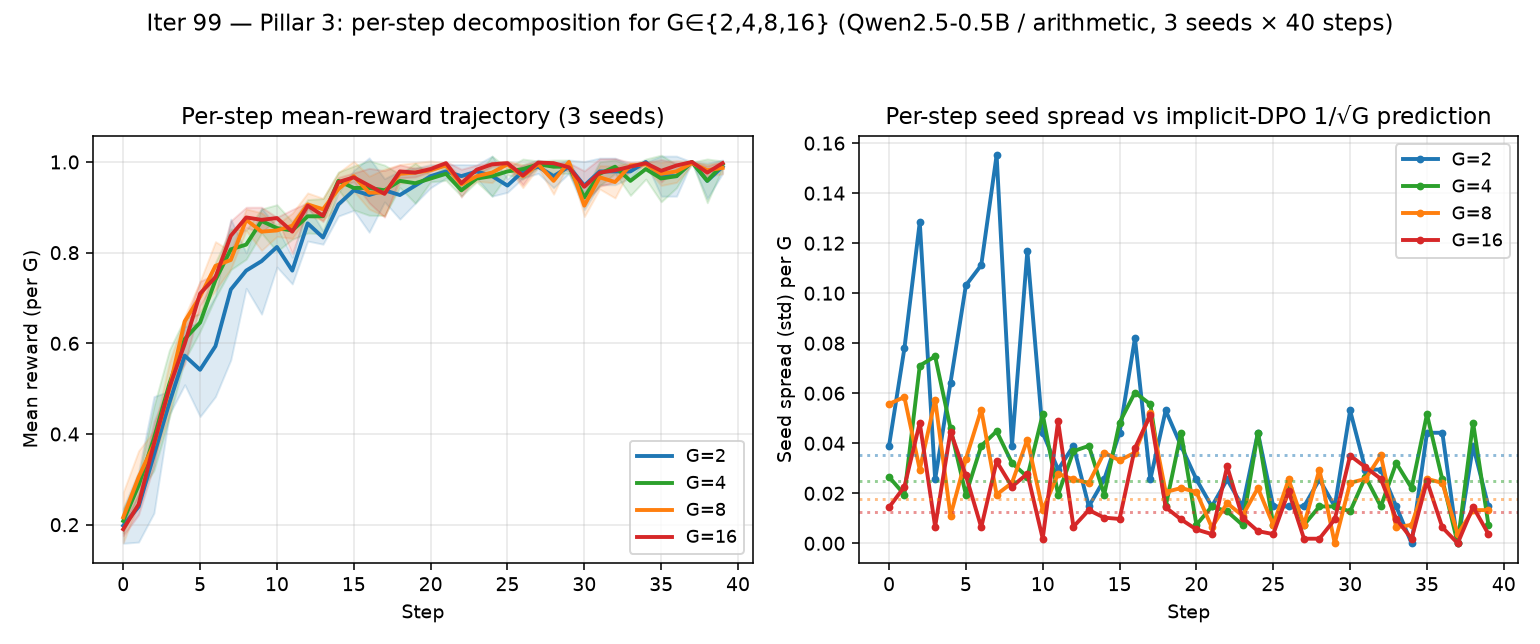
\includegraphics[width=0.95\linewidth]{figures/group_size_iter99.pdf}
  \caption{\textbf{Iter 99 -- per-step decomposition (Qwen2.5-0.5B /
  arithmetic, 3 seeds $\times$ 40 steps).} Left: per-$G$ mean-reward
  trace with shaded seed-spread. Right: per-step seed std of mean
  reward; horizontal dotted lines are the naive
  $1/\sqrt{G}$ prediction scaled to $G{=}16$.  Empirical noise floor
  is non-monotone in $G$ and falls well short of the
  $1/\sqrt{G}$ compression implicit DPO would predict.}
  \label{fig:groupsize-iter99}
\end{figure}
